We can now phrase the correctness properties in \autoref{sec:concepts} in terms
of the QAC language family:
\begin{enumerate}
  \item A rejection-sound ({\it i.e.} acceptance-complete) validator consumes
    all traces that are producible by the protocol specification:
    \[\begin{array}{lrl}
      \rejSound v s&\triangleq&\forall t,\rejects v t\implies\invalid s t\\
      &\triangleq&\forall t,(\exists s',\behaves s t s')\implies\exists v',\behaves v t v'
    \end{array}\]
  \item A rejection-complete ({\it i.e.} acceptance-sound) validator only
    consumes traces that are producible by the protocol specification:
    \[\begin{array}{lrl}
      \rejComplete v s&\triangleq&\forall t,\invalid s t\implies\rejects v t\\
      &\triangleq&\forall t,(\exists v',\behaves v t v')\implies\exists s',\behaves s t s'
    \end{array}\]
\end{enumerate}

Both the specification and the validator are infinite loops.  To show that the
validator consumes the same space of traces as the specification produces, we
need to show the correspondence between each server and validator step.  This is
done by introducing some loop invariant between the server and validator states,
and show that it is preserved by the server's and the validator's loop body.

This section shows how to prove that validator $\existT{V}{\beta}{(\vstep,v_0)}$
is sound and complete with respect to the server model
$\existT{S}{\sigma}{(\sstep,s_0)}$.  The core of the proof is the loop invariant
defined as a binary relation between the validator state $\beta$ and the server
state $\sigma$.  Notation ``$(\Reflects v s)$'' is pronounced ``validator state
$v$ simulates server state $s$''.

\subsection{Proving rejection soundness}
To prove that any trace producible by the server is consumable by the validator,
I perform forward induction on the server's execution path, and show that every
step has a corresponding validator step:

\begin{itemize}
\item The initial server state $s_0$ simulates the initial validator state $v_0$:
  \begin{equation}
    \tag{RejSound-Init}
    \label{eq:rs1}
    \Reflects{v_0}{s_0}
  \end{equation}
\item Any server step $\triggers sc{(q,a)}s'$ whose pre-execution state $s$
  reflects some pre-validation state $v$ can be consumed by the validator
  yielding a post-validation state $v'$ that reflects the post-execution state
  $s'$:
  \begin{align*}
    \tag{RejSound-Step}
    \label{eq:rs2}
    &\forall(q:Q)(c:C)(a:A)(s,s':\sigma)(v:\beta),\\
    &\triggers sc{(q,a)}s'\;\wedge\;\Reflects{v}{s}\\
    &\implies\exists(v':\beta),\;\behaves v{(q,a)}v'\;\wedge\;\Reflects{v'}{s'}
  \end{align*}
  \begin{center}
    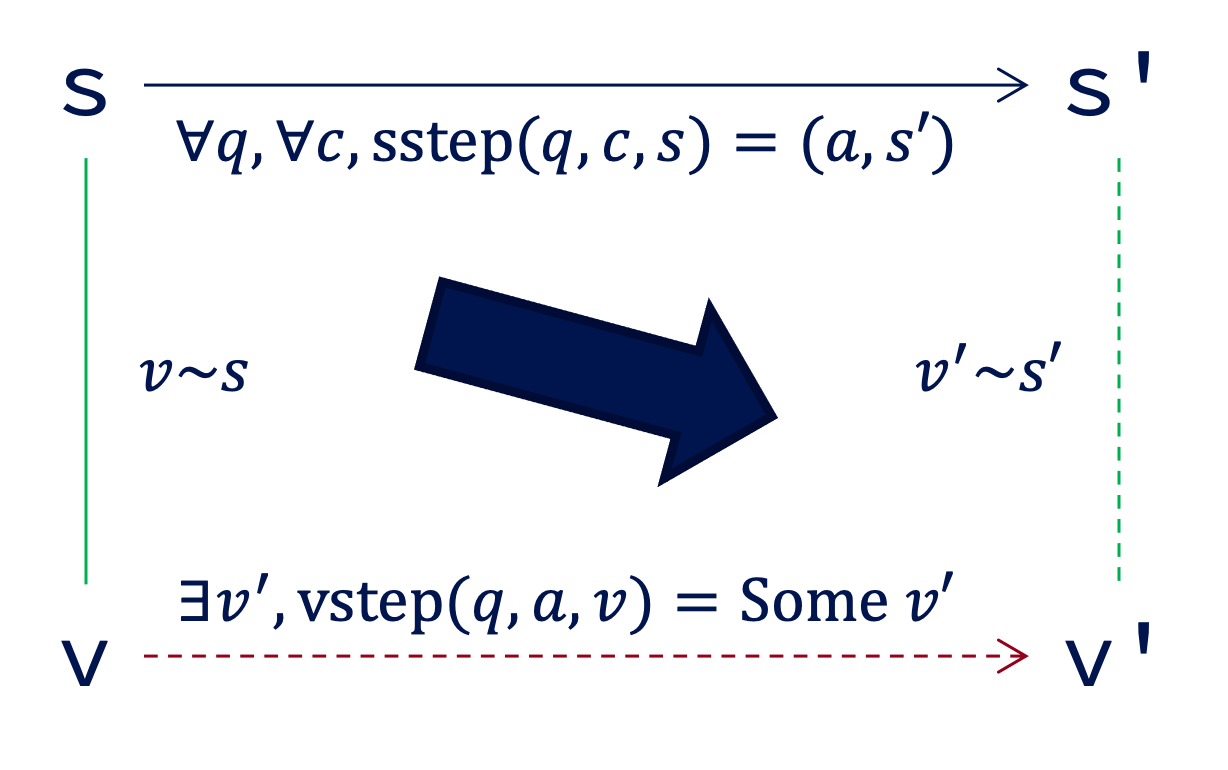
\includegraphics[width=.5\textwidth]{figures/sound}
  \end{center}
\end{itemize}

Here syntax ``$\triggers sc{(q,a)}s'$~'' and ``$\behaves v{(q,a)}v'$~'' are
simplified from \autoref{def:server-step} and \autoref{def:validator-step},
representing the server and validator instances by their states.  This is
because their state types $\sigma,\beta$ and step functions $\sstep,\vstep$
remain constant over the transitions.

\subsection{Proving rejection completeness}
Rejection completeness says that any trace consumable by the validator is
producible by the server model.  I construct the server's execution path
$\behaves sts'$ by {\em backward} induction of the validation path $\behaves
vtv'$:
\begin{itemize}
\item Any accepting validator step $\behaves v{(q,a)}v'$ has some server
  state $s'$ that reflects the post-validation state $v'$:
  \begin{align*}
    \tag{RejComplete-End}
    \label{eq:rc1}
    \forall(q:Q)(a:A)(v, v':\beta),\;&\behaves v{(q,a)}v'\\
    &\implies\exists s':\sigma,\Reflects{v'}{s'} 
  \end{align*}
  This gives us a final server state from which we can construct the server's
  execution path inductively.

\item Any accepting validator step $\behaves v{(q,a)}v'$ whose
  post-validation state $v'$ reflects some post-execution server state $s'$
  has a corresponding server step from a pre-execution state $s$
  that reflects the pre-validation state $v$:
  \begin{align*}
    \tag{RejComplete-Step}
    \label{eq:rc2}
    &\forall(q:Q)(a:A)(v,v':\beta)(s':\sigma),\\
    &\vstep(q,a,v)=\Some{v'}\wedge\Reflects{v'}{s'}\\
    &\implies\exists(s:\sigma)(c:C),\sstep(q,c,s)=(a,s')\wedge\Reflects{v}{s}
  \end{align*}
  \begin{center}
    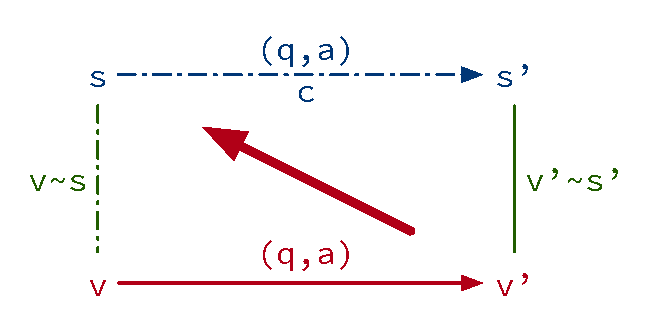
\includegraphics[width=.5\textwidth]{figures/complete}
  \end{center}

\item The initial validator state $v_0$ only reflects the initial server state $s_0$:
  \begin{equation}
    \tag{RejComplete-Init}
    \label{eq:rc3}
    \{s\mid\Reflects{v_0}{s}\}=\{s_0\}
  \end{equation}
\end{itemize}

Rejection soundness is proven by forward induction, while rejection completeness
is proven by backward induction.  This is because the choice $C$ is known from
the server step, but unknown from the validator step: Given a validator step, we
cannot predict ``what choices the server will make in the future'', but can
analyze ``what choices the server might have made in the past''.  This proof
strategy is formalized in the Coq proof assistant, and will be demonstrated with
an example in \autoref{sec:proof}.
